% Created 2017-07-26 Wed 21:02
\documentclass[12pt,article]{article}
\usepackage[utf8]{inputenc}
\usepackage[T1]{fontenc}
\usepackage{fixltx2e}
\usepackage{graphicx}
\usepackage{longtable}
\usepackage{float}
\usepackage{wrapfig}
\usepackage{rotating}
\usepackage[normalem]{ulem}
\usepackage{amsmath}
\usepackage{textcomp}
\usepackage{marvosym}
\usepackage{wasysym}
\usepackage{amssymb}
\usepackage{hyperref}
\tolerance=1000
\newcommand{\T}{\top}
\newcommand{\E}{\ensuremath{\mbox{E}}}
\newcommand{\R}{\ensuremath{\mathbb{R}}}
\newcommand{\one}{\ensuremath{\mathbbm{1}}}
\newcommand{\Eq}[1]{(\ref{eq:#1})}
\renewcommand{\vec}[1]{\boldsymbol{#1}}
\usepackage{biblatex}
\bibliography{prospectus}
\usepackage[style=authordate]{biblatex}
\usepackage{bbm}
\usepackage{dcolumn}\newcolumntype{d}[1]{D{.}{.}{#1}}
\newtheorem{proposition}{Proposition} \newcommand{\Prop}[1]{Proposition \ref{prop:#1}}
\newtheorem{theorem}{Theorem} \newcommand{\Thm}[1]{Theorem \ref{thm:#1}}
\newtheorem{remark}{Remark} \newcommand{\Rem}[1]{Remark \ref{rem:#1}}
\newtheorem{condition}{Condition} \newcommand{\Cond}[1]{Condition \ref{cond:#1}}
\newtheorem{lemma}{Lemma} \newcommand{\Lem}[1]{Lemma \ref{prop:#1}}
\newcommand{\Fig}[1]{Figure \ref{fig:#1}} \newcommand{\Tab}[1]{Table \ref{tab:#1}}
\author{Reajul Chowdhury, Elliott Collins, Ethan Ligon, Munshi Sulaiman}
\date{December 15, 2016}
\title{Valuing Assets Provided to Low-Income Households in South Sudan}
\hypersetup{
  pdfkeywords={},
  pdfsubject={},
  pdfcreator={Emacs 24.5.1 (Org mode 8.2.10)}}
\begin{document}

\maketitle
\begin{abstract}


Several previous studies have found that the ``graduation'' or ``Transfers to the
Ultra-Poor'' (TUP) framework is an effective approach to alleviating the constraints
that prevent extremely poor households from increasing their productivity. The
framework consists of a sizable transfer of productive physical capital, coupled with
training and continuous support over the course of one or two years. A second and
related literature suggests that unconditional cash transfers (UCT's) may have a
comparable effect on productivity and welfare (with fewer fixed costs). This field
experiment, examining the first two years of BRAC's TUP pilot in South Sudan, offers
a direct comparison of these very different approaches to alleviating capital
constraints. We consider the effect of each on consumption, income, asset holdings,
and a number of intangible outcomes. We also consider the TUP program's effect on
households' response to the outbreak of violence in 2014, which led to a level of
instability in which the Graduation framework has not been previously tested. We find
evidence of positive consumption effects from both treatments, but only in the
short-run, and a persistent wealth effect only from the TUP. We also elicit
suggestive evidence that BRAC's support may have helped TUP beneficiaries cope with
the short-term economic effects of the outbreak of violence in 2014. We tentatively
conclude that targeted asset transfers can play a constructive role in helping poor,
self-employed households when they face economic uncertainty. And while cash
increases household consumption, the goal of improving income or wealth is aided by
the additional services that the ultra-poor graduation framework offer.
\end{abstract}
\newpage

\section{Introduction}
\label{sec-1}

Poor rural households typically earn money from low-return activities like
small-scale cultivation or casual day labor, and face both financial and human
capital constraints, keeping them from investing and expanding into more lucrative
activities. Experience and research over many years has lead many to believe that
households facing particularly acute poverty are unable to solve this problem through
the small, high-interest loans typically marketed to them. It was these
considerations that lead to the development of the initial ``Targeting the
Ultra-Poor'' (TUP) program in Bangladesh as a supplement or precursor to credit
services. First implemented by BRAC in 2007, the program aims to simultaneously
alleviate physical and human capital constraints by providing households with a
significant transfer of food and productive assets, followed by two years of training
and support by extension officers. The general framework\footnote{known as the
``graduation framework'' pointing to the original ambition to move households into an
activity where they are able to finance further income growth without costly
transfers.} has since expanded to a wide range of countries, with a general pattern
of success in increasing aggregate investment, labor supply, and aggregate
consumption. (Banerjee et al., 2015) (Bandiera et al., 2016)

A second, older literature has gained new interest in parallel with this
literature which examines the effect of offering direct unconditional cash transfers
(UCT's) to poor households. (Haushoffer \& Shapiro, 2016) (Blattman et al., 2014)
(Blattman et al., 2013) While this and the TUP framework are both direct capital transfer
interventions, they are very different in their approach, with TUP programs guiding
and constraining the use of capital towards productive investment while UCT's allow
households to invest and consume as they see fit. The natural question that arises is
how these additional features and constraints in the TUP framework change how
households use their capital transfers.

Here, we examine the experimental evaluation of BRAC's pilot TUP program in South
Sudan and compare it to a round of unconditional cash transfers. Our results
contribute to the general literature in two important ways. First, South Sudan's
political and economic institutions have overwhelmingly politically unstable since
this study's inception, which may affect the value of the program for
households in important ways. Second, a randomly selected group of households
received cash transfers equal in market value to the assets provided to the TUP
households. While an experimental literature has been established studying the
graduation framework in isolation, this is among the first experiments attempting to
directly compare it to a obvious alternative investment.

\section{The Program}
\label{sec-2}

The pilot program itself was similar to the other TUP programs completed by BRAC. It
consisted of four phases: targeting and selection, training and enterprise selection,
asset transfers, and monitoring. 

\subsubsection{Targeting, Selection, \& Training}
\label{sec-2-0-1}

The fist phase of the program was to complete a census of households in the area
around BRAC's office in the town of Yei in Western Equitoria. This census contained
questions to assess eligibility for the program. First, households were excluded if
they had a salaried worker in the household, were participating in another NGO
program, or had no access to cultivable land (which was in some cases necessary for
the program's model). Households were then deemed eligible if they fit at least three
criteria in a list of five poverty indicators.\footnote{These criteria were that the
household had a head working as a day laborer (generally an occupation with poverty
wages), two or more children, at least one child working, fewer than three rooms, or
a woman who has not completed secondary school.} The census was completed in April of
2013 and 745 were identified as eligible. Of these, 649 were identified in a baseline
survey. These households were stratified on employment, asset ownership, and size and
selected into treatment groups. 250 were enrolled in the TUP program, 125 in the UCT
group, and the final 274 in a pure control group.

\subsubsection{Asset Transfers \& Monitoring}
\label{sec-2-0-2}

The second phase of the program was training and enterprise selection. Unlike most
programs of this type, the number of households given each kind of asset was set in
advance, with 75 enrolled in agricultural activities (vegetable cultivation), 85 in
duck rearing, 45 in goat rearing, and the rest in small trade businesses. While the
staff tried to map housheolds' asset types to their respective preferences and
skills, a disproportionate number stated a preferences for goats and small trade.
Households then atttended training sessions. The first of these were for general
business skills around literacy, numercacy, and financial management. The next were
sector specific and focused on how to properly raise livestock or gardens. 

Once training is completed, asset transfers began in late 2013 and continued through
the first few months of 2014. The productive assets related to each enterprise were
valued at around \$240 per household, with a random subset recieving an additional \$60
in assets later in 2014. Shortly thereafter, households started to attend weekly or
semi-weekly meetings with other nearby participants to discuss with each other and a
BRAC extension officer the details of their businesses. These meetings also included
food transfers for a while, which were designed to help get households to the point
of receiving revenue from their assets without having to sell them.

In all, the market value of these food transfers were valued at \$110, bringing the
total value of all transfers to \$350-\$410. The 125 households in the UCT group were
randomly divided in half to receive cash in these amounts. Unfortunately, political
instability disrupted NGO operations throughtout South Sudan, preventing the
simultaneous disbursal of the cash and asset transfers. Instead, a second survey was
conducted in June of 2014, with the cash transfers being disbursed immediately
thereafter. This resulted in a timing difference of 3 to 6 months between the two.

\subsection{The Data}
\label{sec-2-1}

The census was conducted in April of 2013 in the area around BRAC's offices in Yei
County to identify women eligible for participation. A baseline survey was conducted
that Summer, which successfully interviewed 649 of these women and randomly selected
them into the TUP, UCT, and control groups. Half of each beneficiary group was
randomly selected to receive additional "top-up" transfers with market value of \$60
(around 20\% of the original transfers).

In response to the outbreak of violence in late 2013 and subsequent closing of the
offices in Yei, a midline survey was conducted in June 2014 to try to separate pre-
and post-conflict changes in outcomes. For lack of a valid comparison group, we will
not speak with any authority about the effect of the conflict on economic conditions
in Yei, though we will report estimates of treatment effects on the severity or
likelihood of having been effected exposure to the conflict. Some of the original
asset transfers were done before the office closure, which may affect estimates of
the difference between programs if rates of return changed in the few intervening
months. Finally, an endline survey was conducted in mid-2015 to estimate the effect
of program participation on households' financial situation and overall welfare. The
key here is that the survey conducted in mid-2014 provides us with \emph{short-term}
treatment effects of the TUP program within 6 months of the asset transfers, while
providing a second baseline for the Cash transfers. Likewise, the 2015 survey
allows us to estimate treatment effects one year after the cash transfers, and 15-18
months after the asset transfers.

This unfortunately left us without data past one year for the cash transfer effects.
To get some point estimates on household welfare for this group in the slightly
longer term, we conducted a series of five short surveys on a monthly basis from
November of 2015 to March of 2016. These collected only a subset of the full
consumption modules and a few questions tracking major transactions and shocks. The
short length of the survey allowed them to be administered via the mobile network,
reducing cost and improving response rate.

\subsection{Empirical Strategy}
\label{sec-2-2}

For the main panel, we estimate a single model using interactions between time effects and group
assignment, as well as baseline values of the outcome variable where available. 

\begin{equation*}
Y_{it} =\sum_{t=2014}^{2015}\delta_{t}+\beta_{t}^{Cash}I_{t}*Cash_{it}+\beta_{t}^{TUP}I_{t}*TUP_{it}+\gamma Y_{i,2013}+\epsilon_{i}
\end{equation*}

where $\delta_{t}$ are time fixed effects and $I_{t}$ is an indicator if the year
\emph{t}, and $Y_{it}$ is an outcome of interest for household \emph{i} in year \emph{t}. We take
the interactions of TUP assignment with 2014 and 2015 indicators as the treatment
effects at 6-8 and 15-17 months respectively. The analagous interactions with the
Cash group offer a second baseline and a 12-month treatment effect, respectively.
Since those transfers happened after the midline survey, its interaction with \emph{2014}
acts as a placebo; there is no \emph{ex ante} reason to expect that they were different
from the rest of the control group at that point. Given the slight difference in
timing, we report a t-test of the hypothesis $\beta$$_{\text{TUP,t}}$-$\beta$$_{\text{Cash,2015}}$=0 for
both \(t \in {2014,2015}\). Since the difference in timing is much smaller, we consider
\(\beta_{TUP,2015}-\beta_{Cash,2015}=0\) to be the central hypothesis of interest.

For the supplementary analysis of the high-frequency panel, we estimate a separate
model, since the underlying data is so different. A constant parameter takes the
place of the fixed effects. We include 2013 levels as a covariate where possible.
Since we collect expenditures on only ten consumption items, we report not only the
total value of spending on those goods, but also a more theoretically grounded
measure described in Collins \& Ligon (2017), which uses the composition of
expenditures to derive the marginal utility of expenditures for each household. We
chose ten relatively demand-elastic items specifically for this purpose, as those
will tend to be the most responsive to changes in welfare.

\section{Results}
\label{sec-3}
\subsection{Randomization Check}
\label{sec-3-1}

A crucial assumption is that the treatment and control groups were selected
appropriately. We check this by presenting summary statistics by group on a
range of factors related to consumption, asset holdings, and household
characteristics. We check for balance on observables in Table 1.

\begin{longtable}{lrrrrr}
\caption{\label{tab:balance_check}Means of some analysis variables at baseline.  Asterisks indicate p<.1, .05, and .01 respectively}
\\
\hline
Consumption & CTL & $\Delta$ TUP & $\Delta$ CSH & $N$\\
\hline
\endhead
\hline\multicolumn{5}{r}{Continued on next page} \\
\endfoot
\endlastfoot
Meat & 4.21 & -0.568 & -0.052 & 378\\
Fuel & 0.76 & -0.039 & -0.072 & 456\\
Clothesfootwear & 0.67 & -0.026 & 0.033 & 595\\
Soap & 0.48 & -0.008 & -0.026 & 536\\
Fish & 2.50 & -0.154 & -0.156 & 474\\
Charities & 0.03 & -0.006 & 0.0 & 134\\
Cereals & 9.19 & -0.947 & 0.27 & 605\\
Transport & 0.18 & -0.033 & 0.002 & 193\\
Cosmetics & 0.68 & 0.027 & -0.125 & 468\\
Sugar & 1.71 & -0.078 & -0.189 & 604\\
Egg & 1.10 & -0.091 & 0.038 & 276\\
Oil & 1.36 & -0.13 & -0.141 & 613\\
CSH & 0.00 & 0.0 & 1.0 & 125\\
Ceremonies & 0.13 & 0.006 & 0.026 & 152\\
Beans & 0.70 & 0.232 & 0.226 & 192\\
Fruit & 0.69 & -0.089 & 0.001 & 272\\
Textiles & 0.16 & -0.004 & 0.056$^{\text{*}}$ & 376\\
Utensils & 0.25 & -0.009 & 0.008 & 442\\
Dowry & 1.27 & -0.041 & 0.028 & 126\\
Furniture & 0.20 & -0.014 & 0.045 & 368\\
TUP & 0.00 & 1.0 & 0.0 & 249\\
Salt & 0.45 & -0.026 & 0.007 & 617\\
Vegetables & 1.54 & -0.165 & -0.18 & 471\\
\hline
Assets & CTL & $\Delta$ TUP & $\Delta$ CSH & $N$\\
\hline
Smallanimals & 236.60 & -86.068 & -123.133 & 123\\
Bicycle & 109.08 & -12.555 & -11.414 & 171\\
CSH & 0.00 & 0.0 & 1.0 & 125\\
Radio & 58.45 & -5.968 & -16.529 & 260\\
Motorcycle & 341.74 & 192.956 & 353.836$^{\text{**}}$ & 93\\
TUP & 0.00 & 1.0 & 0.0 & 249\\
Net & 19.16 & 0.668 & 0.247 & 423\\
Poultry & 42.40 & -3.365 & -8.894 & 161\\
Bed & 241.27 & 7.992 & 32.762 & 521\\
Chairtables & 206.79 & -29.368 & 3.617 & 531\\
Mobile & 97.54 & 12.627 & -4.198 & 414\\
Netitn & 7.82 & 1.215 & 1.178 & 181\\
Cosmetics & 0.68 & 0.027 & -0.125 & 468\\
\hline
Household & CTL & $\Delta$ TUP & $\Delta$ CSH & $N$\\
\hline
Daily Food & 25.18 & -2.215 & -0.261 & 643\\
Daily Exp & 29.90 & -2.167 & -0.288 & 646\\
No. Houses & 2.83 & 0.031 & 0.118 & 543\\
In Business & 0.40 & 0.038 & 0.017 & 265\\
Cereals & 9.19 & -0.947 & 0.27 & 605\\
\# Child & 3.26 & 0.118 & 0.108 & 594\\
Asset Tot. & 1757.05 & -44.791 & 98.654 & 603\\
Cash Savings & 236.90 & 28.52 & -66.812 & 431\\
HH size & 7.23 & -0.175 & 0.3 & 648\\
\hline
\end{longtable}

This is simply suggestive evidence that the treatment and control groups were similar
in observables at baseline, with the exception that the cash group has atypically
more motorcycles and clothing. But it does suggests that our stratified randomization
was not too far from creating comparable groups.

\subsection{Consumption}
\label{sec-3-2}

The first measure of welfare we consider is household consumption, defined as the
market value of goods or services used by the household. A sizable basket of goods
were included in the survey module. These are separated into three categories: Food
items (with a 3-day recall window), non-durables (a 30-day recall window), and
durables and large expenditures (a one-year recall window). This is perhaps the most
appropriate measure of the welfare or poverty of a household in our survey. 

The results for several important consumption measures are presented in Table
\ref{tab:consumption}. Importantly, we do not know about prices for each good in this
time, though we can say that inflation was as high as 100\% between 2014 and 2015.
Nonetheless, we take the sum of all consumption and expenditure questions together as
a measure of welfare. In light of the fact that we have data on an incomplete basket, we also
follow Collins and Ligon (2015), which details a method for deriving treatment
effects on a model-based estimate of households' marginal utility, which we include
here as \(\log\lambda_{it}\).

The main result is that TUP participants had higher consumption consumption in 2014,
several months into the primary monitoring phase after the asset transfers.
Similarly, the cash group has higher consumption in 2015, measured just over a year
after disbursal. Food transfers had ceased weeks before the 2014 survey was
conducted, and the assets had been transferred 6-8 months prior. The TUP group sees
no notable effect in 2015. The short-term consumption effects of either program are
economically significant, representing a roughly 16\% increase in average total
consumption for both TUP and Cash. These results are consistent with a story in which
either sort of transfer has a short-term consumption effect. Importantly, we do not
reject the null hypothesis that the two effects are equal to one another. In either
group, the increase in total consumption appears to be driven mainly by increased
food consumption, with smaller effects on non-food consumption goods and durables. As
such, there is no evidence that the share of food consumed falls, as might be
predicted by Engel's law.

\newpage

\begin{longtable}{lrrrrrrr}
\caption{\label{tab:consumption}Average treatment effects by Group-Year, controlling for baseline levels.}
\\
\hline
 & Tot & $\log\lambda_{it}$ & Food & logTot\\
\hline
\endhead
\hline\multicolumn{5}{r}{Continued on next page} \\
\endfoot
\endlastfoot
CTL mean & $115.404$ & $0.159$ & $38.468$ & $4.509^{***}$\\
 & $(78.750)$ & $(0.967)$ & $(26.250)$ & $(0.756)$\\
\hline
CSH*2014 & $-2.745$ & $0.127$ & $-0.915$ & $0.007$\\
 & $(8.008)$ & $(0.110)$ & $(2.669)$ & $(0.079)$\\
CSH*2015 & $18.023^{**}$ & $-0.145$ & $6.008^{**}$ & $0.160^{**}$\\
 & $(7.831)$ & $(0.108)$ & $(2.610)$ & $(0.077)$\\
TUP*2014 & $18.590^{***}$ & $-0.365^{***}$ & $6.197^{***}$ & $0.212^{***}$\\
 & $(6.426)$ & $(0.089)$ & $(2.142)$ & $(0.063)$\\
TUP*2015 & $4.179$ & $-0.055$ & $1.393$ & $0.045$\\
 & $(6.130)$ & $(0.084)$ & $(2.043)$ & $(0.060)$\\
2014 & $76.831^{***}$ & $0.214^{***}$ & $25.610^{***}$ & $3.931^{***}$\\
 & $(5.318)$ & $(0.062)$ & $(1.773)$ & $(0.113)$\\
2015 & $105.702^{***}$ & $0.188^{***}$ & $35.234^{***}$ & $4.175^{***}$\\
 & $(5.001)$ & $(0.057)$ & $(1.667)$ & $(0.111)$\\
Bsln2013 & $0.081^{**}$ & $0.022$ & $0.081^{**}$ & $0.073^{***}$\\
 & $(0.038)$ & $(0.029)$ & $(0.038)$ & $(0.026)$\\
Bsln$_{\text{NAN}}$ & $20.521^{***}$ & $-0.119$ & $6.840^{***}$ & $0.447^{***}$\\
 & $(6.964)$ & $(0.088)$ & $(2.321)$ & $(0.121)$\\
\hline
$\beta^{TUP}_{2014}-\beta^{CSH}$ & $0.566$ & $-0.220$ & $0.189$ & $0.052$\\
 & $(9.994)$ & $(0.137)$ & $(3.331)$ & $(0.098)$\\
$\beta^{TUP}_{2015}-\beta^{CSH}$ & $-13.844^{*}$ & $0.090$ & $-4.615^{*}$ & $-0.115$\\
 & $(8.125)$ & $(0.111)$ & $(2.708)$ & $(0.080)$\\
\hline
F-stat & $10.142$ & $4.169$ & $10.142$ & $8.131$\\
N & $1291.000$ & $1296.000$ & $1291.000$ & $1291.000$\\
\hline
\end{longtable}


This result leaves open the question of whether the cash treatment had a persistent effect
on consumption, or whether the short-term effect found in 2015 is similarly
temporary. It was this question that motivated the collection of an additional five
rounds of data over a 6-month period in late 2015 and early 2016, in which
we asked about ten items, five food and five non-food. We consider the average treatment effect
on households sampled for these phone interviews, both for $\log$$\lambda$$_{\text{it}}$ and for
"Total consumption", which in this case we take a simple sum over the goods
discussed. We find that, consistent with the TUP program's results in 2015, all evidence of an effect
seem to be gone by 18th months after the transfer date.

\begin{longtable}{lrrrrr}
\caption{\label{tab:mobile_consumption}Average treatment effects using mobile data collection (results are robust to controlling for baseline levels)}
\\
\hline
 & $\log\lambda_{it}$ & Tot & logTot\\
\hline
\endhead
\hline\multicolumn{4}{r}{Continued on next page} \\
\endfoot
\endlastfoot
CTL mean & $-0.018$ & $30.851$ & $3.158^{***}$\\
 & $(1.001)$ & $(27.768)$ & $(0.734)$\\
\hline
TUP & $0.023$ & $-0.624$ & $-0.011$\\
 & $(0.041)$ & $(1.152)$ & $(0.030)$\\
CSH & $0.056$ & $0.776$ & $0.028$\\
 & $(0.052)$ & $(1.459)$ & $(0.038)$\\
const & $-0.018$ & $30.851^{***}$ & $3.158^{***}$\\
 & $(0.027)$ & $(0.753)$ & $(0.020)$\\
\hline
$\beta^{TUP}-\beta^{CSH}$ & $-0.033$ & $-1.399$ & $-0.039$\\
 & $(0.055)$ & $(1.524)$ & $(0.040)$\\
\hline
F-stat & $0.584$ & $0.434$ & $0.475$\\
N & $2877.000$ & $2878.000$ & $2878.000$\\
\hline
\end{longtable}


\subsection{Food Security}
\label{sec-3-3}

Generally speaking, observed changes in total consumption don't translate into an
increase in reported food security. In each year, we ask how often in a given week
the respondent has had experiences indicative of food insecurity. Included are (from
left to right) going a whole day without eating, going to sleep hungry, being without
any food in the house, eating fewer meals than normal at mealtimes, and limiting
portions. We report the percentage of people who report experiencing each in a
typical week, as well as a standardized composite z-score using all of these
questions. There is little evidence of a significant treatment effect at endline
in 2015.

\begin{longtable}{lrrrrrrr}
\caption{\label{tab:foodsecure}Percentage of respondents reporting a food security problem occurs at least once a week.}
\\
\hline
 & Z-score & Whole Day & Hungry & No Food & Fewmeals & Portions\\
\hline
\endhead
\hline\multicolumn{7}{r}{Continued on next page} \\
\endfoot
\endlastfoot
CTL mean & $-0.01$ & \$ 0.21\$ & \$ 0.21\$ & \$ 0.28\$ & \$ 0.32\$ & \$ 0.36\$\\
 & $( 1.00)$ & $( 0.41)$ & $( 0.40)$ & $( 0.45)$ & $( 0.47)$ & $( 0.48)$\\
\hline
TUP*2014 & $-0.10$ & $-0.02$ & $-0.05$ & $-0.03$ & \$ 0.01\$ & \$ 0.01\$\\
 & $( 0.09)$ & $( 0.03)$ & $( 0.03)$ & $( 0.03)$ & $( 0.04)$ & $( 0.04)$\\
TUP*2015 & $-0.02$ & \$ 0.03\$ & $-0.01$ & $-0.03$ & \$ 0.05\$ & $-0.02$\\
 & $( 0.09)$ & $( 0.03)$ & $( 0.03)$ & $( 0.03)$ & $( 0.04)$ & $( 0.04)$\\
CSH*2014 & $-0.05$ & $-0.00$ & $-0.04$ & $-0.01$ & $-0.03$ & $-0.00$\\
 & $( 0.11)$ & $( 0.04)$ & $( 0.04)$ & $( 0.04)$ & $( 0.05)$ & $( 0.05)$\\
CSH*2015 & \$ 0.03\$ & \$ 0.06\$ & \$ 0.03\$ & $-0.01$ & $-0.00$ & $-0.04$\\
 & $( 0.11)$ & $( 0.04)$ & $( 0.04)$ & $( 0.04)$ & $( 0.05)$ & $( 0.05)$\\
Bsln2013 & \$ 0.07$^{\text{**}}$\$ & $-0.00$ & \$ 0.02\$ & \$ 0.03\$ & \$ 0.06$^{\text{**}}$\$ & $-0.02$\\
 & $( 0.03)$ & $( 0.02)$ & $( 0.02)$ & $( 0.02)$ & $( 0.03)$ & $( 0.03)$\\
2014 & \$ 0.07\$ & \$ 0.09$^{\textbf{*}}$\$ & \$ 0.10$^{\textbf{*}}$\$ & \$ 0.09$^{\textbf{*}}$\$ & \$ 0.17$^{\textbf{*}}$\$ & \$ 0.22$^{\textbf{*}}$\$\\
 & $( 0.06)$ & $( 0.02)$ & $( 0.02)$ & $( 0.03)$ & $( 0.03)$ & $( 0.03)$\\
2015 & \$ 0.03\$ & \$ 0.22$^{\textbf{*}}$\$ & \$ 0.21$^{\textbf{*}}$\$ & \$ 0.26$^{\textbf{*}}$\$ & \$ 0.30$^{\textbf{*}}$\$ & \$ 0.39$^{\textbf{*}}$\$\\
 & $( 0.06)$ & $( 0.02)$ & $( 0.02)$ & $( 0.02)$ & $( 0.03)$ & $( 0.03)$\\
Bsln$_{\text{NAN}}$ & $-0.17^{*}$ & $-0.02$ & $-0.03$ & \$ 0.03\$ & $-0.02$ & $-0.08^{*}$\\
 & $( 0.09)$ & $( 0.03)$ & $( 0.03)$ & $( 0.03)$ & $( 0.04)$ & $( 0.04)$\\
\hline
F-stat & \$ 1.45\$ & \$ 9.34\$ & \$ 8.36\$ & $10.84$ & \$ 6.70\$ & \$ 5.91\$\\
N & $1299.00$ & $1282.00$ & $1297.00$ & $1293.00$ & $1297.00$ & $1292.00$\\
\hline
$\beta^{TUP}_{2014}-\beta^{CSH}$ & $-0.13$ & $-0.08$ & $-0.08^{*}$ & $-0.01$ & \$ 0.01\$ & \$ 0.05\$\\
 & $( 0.14)$ & $( 0.05)$ & $( 0.05)$ & $( 0.05)$ & $( 0.06)$ & $( 0.06)$\\
$\beta^{TUP}_{2015}-\beta^{CSH}$ & $-0.06$ & $-0.03$ & $-0.04$ & $-0.02$ & \$ 0.06\$ & \$ 0.02\$\\
 & $( 0.12)$ & $( 0.04)$ & $( 0.04)$ & $( 0.04)$ & $( 0.05)$ & $( 0.05)$\\
\hline
\end{longtable}

\subsection{Assets}
\label{sec-3-4}

Turning now to asset holdings for the households, we estimate treatment effects for total value of assets owned, total
value of potentially productive assets, as well as land and financial assets. 

\subsubsection{Total Asset Holdings}
\label{sec-3-4-1}

The cash group does not appear to have seen an increase in the
value of assets measured, with negative and imprecise point estimates. The most
important result is that the TUP group has significantly more asset wealth than the
cash or control groups in both 2014 and 2015, 18 months after receipt of transfers.
The TUP group has a change of 536 SSP on average (43\% increase over controls, p<.01).
So-called "Productive" assets include anything that could plausibly be used in
productive activity. \footnote{For now, we include in this list: small and large
livestock, farm equipment, mobiles, carts, sewing equipment, sheds, and shop
premises.} Here we see the TUP group has 320 SSP (95\%) more in this area over the
control group, with a similar magnitude at midline.

Importantly, this is not due to a preciptous increase in assets reported over this
time. Note also that the effect on total assets is higher in absolute value than the
effect on productive asset value, suggesting that the increased wealth cannot be
explained purely by households holding onto asset transfers for the length of the
program's monitoring phase. Instead, the TUP group is the only one for whom total
measured asset holdings did not fall on average over these two years, which saw
hyperinflation and a significant aggregate economic downturn. This asset effect
(including the savings effect below) is the only feature of households' financial
situation on which we we see a persistent effect.

\begin{figure}[htb]
\centering
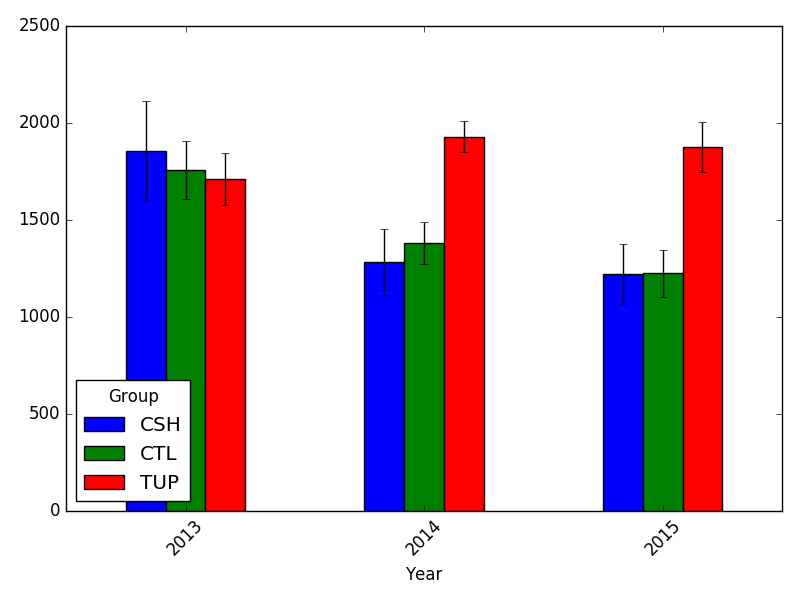
\includegraphics[width=.9\linewidth]{../figures/AssetTotal_groupyear.png}
\caption{\label{fig:AssetTotal}Measured asset wealth by group-year}
\end{figure} 

\begin{longtable}{lrrrrrrr}
\caption{\label{tab:assets}Average treatment effects by group-year on total value (in SSP) of all assets measured and of productive assets measured}
\\
\hline
 & Total & Productive\\
\hline
\endhead
\hline\multicolumn{3}{r}{Continued on next page} \\
\endfoot
\endlastfoot
CTL mean & $1225.61$ & $337.60$\\
 & $(1502.46)$ & $(605.57)$\\
\hline
TUP*2014 & $535.79^{***}$ & $361.80^{***}$\\
 & $(154.02)$ & $(74.19)$\\
TUP*2015 & $624.79^{***}$ & $320.74^{***}$\\
 & $(146.01)$ & $(68.68)$\\
CSH*2014 & $-125.86$ & $18.50$\\
 & $(191.31)$ & $(95.80)$\\
CSH*2015 & $-49.99$ & $-5.00$\\
 & $(187.32)$ & $(88.40)$\\
Bsln2013 & \$ 0.08$^{\textbf{*}}$\$ & \$ 0.00\$\\
 & $( 0.02)$ & $( 0.01)$\\
2014 & $1259.75^{***}$ & $465.53^{***}$\\
 & $(112.68)$ & $(55.96)$\\
2015 & $1124.61^{***}$ & $392.97^{***}$\\
 & $(103.46)$ & $(50.21)$\\
Bsln$_{\text{NAN}}$ & $21.30$ & $-131.14^{**}$\\
 & $(146.51)$ & $(51.35)$\\
\hline
N & $1305.00$ & $1247.00$\\
F-stat & \$ 8.53\$ & $10.19$\\
\hline
$\beta^{TUP}_{2014}-\beta^{CSH}$ & $585.78^{**}$ & $366.79^{***}$\\
 & $(239.76)$ & $(114.58)$\\
$\beta^{TUP}_{2015}-\beta^{CSH}$ & $674.78^{***}$ & $325.74^{***}$\\
 & $(194.72)$ & $(92.26)$\\
\hline
\end{longtable}


\subsubsection{Savings}
\label{sec-3-4-2}

Both treatment arms had significant impact on the average value of cash savings
within households in 2015. The TUP households are strongly encouraged to pay into a savings
account maintained by BRAC each time they meet. Anecdotally, this has discouraged
some women from attending the meetings, but it results in TUP participants being 44\%
(20 pp) more likely to report having any savings at all. It's
worth noting though that since the TUP households also regard their savings behavior
as much more transparent to BRAC (and have received pressure to save from them) than
the other groups, these households may simply be more likely to reveal that they are
saving when asked. Among those who have savings, TUP households report having roughly
43\% (81 SSP) more in value.

Cash households appear no more likely than the control households to report having
cash savings (around 45\% in each group), but households that report having any
savings at all report
having 47\% (91.4 SSP) more in value. This is significantly less than was given to
these households, but combined with the short-term consumption results, goes some
distance in explaining the lack of effect on physical asset wealth. The cash seems to
have gone primarily to consumption and savings.

It is common in this community (and most in the region) to store non-perishable food
like maize, cassava, or millet as a form of savings. This would seem particularly
reasonable in a high-inflation context, where the price of grain had doubled in the
previous year. At least as many households report saving in food (53\%) as in cash
(46\%), with an average market value of 106 SSP. However, we find no evidence that
either treatment group increased food savings. \footnote{Note that food savings was not
measured at baseline, so these controls are omitted.}

Neither do we find evidence that either treatment increased the size or likelihood of
giving or receiving interhousehold transfers, either in cash or in kind. These
results are omitted since only 35 and 60 households reported giving and recieving
transfers respectively, with no difference in group means.

\begin{longtable}{lrrrrrrr}
\caption{\label{tab:Nonzero}Average treatment effects by group-year on percentage of households reporting any savings or land access}
\\
\hline
\% > 0 & Savings & Food Sav & LandCult & LandOwn\\
\hline
\endhead
\hline\multicolumn{5}{r}{Continued on next page} \\
\endfoot
\endlastfoot
CTL mean & \$ 0.45\$ & \$ 0.82\$ & \$ 0.82\$ & \$ 0.90\$\\
\hline
CSH*2014 & $-0.06$ & \$ 0.00\$ & $-0.04$ & $-0.01$\\
 & $( 0.06)$ & $( 0.04)$ & $( 0.04)$ & $( 0.04)$\\
CSH*2015 & \$ 0.03\$ & \$ 0.02\$ & \$ 0.05\$ & \$ 0.02\$\\
 & $( 0.05)$ & $( 0.04)$ & $( 0.04)$ & $( 0.04)$\\
TUP*2014 & \$ 0.22$^{\textbf{*}}$\$ & $-0.02$ & $-0.03$ & $-0.00$\\
 & $( 0.04)$ & $( 0.03)$ & $( 0.03)$ & $( 0.03)$\\
TUP*2015 & \$ 0.21$^{\textbf{*}}$\$ & $-0.03$ & \$ 0.01\$ & $-0.01$\\
 & $( 0.04)$ & $( 0.03)$ & $( 0.03)$ & $( 0.03)$\\
2014 & \$ 0.43$^{\textbf{*}}$\$ & \$ 1.00$^{\textbf{*}}$\$ & \$ 0.83$^{\textbf{*}}$\$ & \$ 0.82$^{\textbf{*}}$\$\\
 & $( 0.04)$ & $( 0.02)$ & $( 0.06)$ & $( 0.05)$\\
2015 & \$ 0.39$^{\textbf{*}}$\$ & \$ 0.82$^{\textbf{*}}$\$ & \$ 0.77$^{\textbf{*}}$\$ & \$ 0.84$^{\textbf{*}}$\$\\
 & $( 0.04)$ & $( 0.02)$ & $( 0.05)$ & $( 0.05)$\\
Bsln2013 & \$ 0.05\$ &  & \$ 0.05\$ & \$ 0.07\$\\
 & $( 0.04)$ &  & $( 0.05)$ & $( 0.04)$\\
Bsln$_{\text{NAN}}$ & \$ 0.08$^{\text{*}}$\$ &  & \$ 0.05\$ & \$ 0.05\$\\
 & $( 0.04)$ &  & $( 0.06)$ & $( 0.05)$\\
\hline
$\beta^{TUP}_{2014}-\beta^{CSH}$ & \$ 0.19\$ & $-0.04$ & $-0.07$ & $-0.02$\\
$\beta^{TUP}_{2015}-\beta^{CSH}$ & \$ 0.18\$ & $-0.05$ & $-0.03$ & $-0.03$\\
\hline
F-stat & \$ 8.83\$ & $15.60$ & \$ 0.79\$ & \$ 0.76\$\\
N & $1259.00$ & $870.00$ & $1231.00$ & $1251.00$\\
\hline
\end{longtable}


\begin{longtable}{lrrrrrrr}
\caption{\label{tab:Savings}Average treatment effects by group-year on total value (in SSP) of all cash and food savings and area (in fedan) of land being cultiviated by the household (including rented or temporary-use) and owned by the household.}
\\
\hline
Amt. & Savings & Food Sav & LandCult & LandOwn\\
\hline
\endhead
\hline\multicolumn{5}{r}{Continued on next page} \\
\endfoot
\endlastfoot
CTL mean & $191.19$ & $114.78$ & $61.88$ & $46.00$\\
\hline
CSH*2014 & $28.74$ & \$ 0.22\$ & $10.18$ & $10.50$\\
 & $(42.93)$ & $(15.38)$ & $(15.07)$ & $(12.57)$\\
CSH*2015 & $91.40^{**}$ & $-14.34$ & $-39.18^{***}$ & $-32.37^{***}$\\
 & $(40.89)$ & $(14.98)$ & $(14.90)$ & $(11.95)$\\
TUP*2014 & $-27.09$ & $17.16$ & $-4.76$ & $-3.02$\\
 & $(29.76)$ & $(12.33)$ & $(11.94)$ & $(10.04)$\\
TUP*2015 & $81.33^{***}$ & \$ 1.13\$ & $-17.38$ & $-12.56$\\
 & $(29.32)$ & $(12.26)$ & $(11.65)$ & $( 9.41)$\\
2014 & $106.72^{***}$ & $62.03^{***}$ & $11.37$ & $17.31^{**}$\\
 & $(24.85)$ & $( 8.36)$ & $( 9.94)$ & $( 8.56)$\\
2015 & $163.04^{***}$ & $114.78^{***}$ & $61.52^{***}$ & $51.89^{***}$\\
 & $(24.13)$ & $( 7.60)$ & $( 9.54)$ & $( 7.88)$\\
Bsln2013 & \$ 0.05$^{\text{**}}$\$ &  & \$ 0.94\$ & $-2.43$\\
 & $( 0.02)$ &  & $( 3.07)$ & $( 1.95)$\\
Bsln$_{\text{NAN}}$ & $40.07^{*}$ &  & $-1.60$ & $-6.02$\\
 & $(21.24)$ &  & $( 9.92)$ & $( 8.29)$\\
\hline
$\beta^{TUP}_{2014}-\beta^{CSH}$ & $-118.49$ & $31.50$ & $34.42$ & $29.35$\\
$\beta^{TUP}_{2015}-\beta^{CSH}$ & $-10.07$ & $15.47$ & $21.79$ & $19.80$\\
\hline
F-stat & \$ 7.41\$ & \$ 7.14\$ & \$ 4.91\$ & \$ 3.72\$\\
N & $671.00$ & $777.00$ & $1042.00$ & $1114.00$\\
\hline
\end{longtable}


\subsubsection{Land Holdings}
\label{sec-3-4-3}

We also examine land ownership and cultivation in each year. We find no evidence that
either group is more or less likely to report owning or cultivating at least some land, though this
may be in part because land ownership and cultivation is already very common.
Anecdotaly, divesting from land ownership entirely could be seen as a relatively
drastic decision. 
However, members of the cash group who are involved in agriculture are found to be
cultivating significantly less land after the fact, which reports cultivating 65\%
less and owning 70\% less land than the control group. This raises the interesting
question of whether the cash group was likely to switch occupations from farming to
non-farm self-employment.
It could also raise questions around the underlying logic of the more agrarian
transfer in the TUP program, if unconstrained transfers prompt households to divest
from these opportunities. This concern may be validated somewhat by the fact that TUP
participants primarily stated a preference for small retail training and transfers
over small animal husbandry or vegetable gardening.

\subsection{Income}
\label{sec-3-5}

Income was reliably measured only in 2015, and so our estimates do not control for
baseline values. The control group in 2015 has a measured income of roughly 4325 SSP
per year, or roughly \$540 US (assuming an exchange rate of around 8). The TUP group
sees a 327 SSP (\$41 US, 7\%) increase in annual average income, but with a fairly
skewed distribution and high standard errors. The related figure shows that total
income is not particularly different among groups. Perhaps the main lesson is that
the TUP group has measurably more reported livestock-related income, and less farm
income, indicating a shift away from farming. The cash group may exhibit some
substitution away from farm and livestock, but as is evident graphically, we do not
observe sizable changes in total income for either treatment group. 

\begin{figure}[htb]
\centering
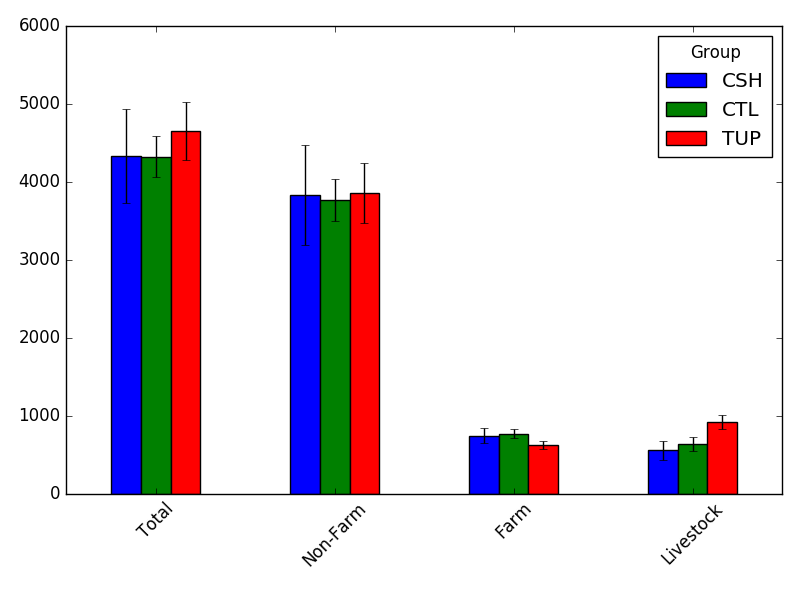
\includegraphics[width=.9\linewidth]{../figures/Income_group.png}
\caption{\label{fig:Income_group}Distribution of total observed income by group}
\end{figure} 



\begin{longtable}{lrrrrrrr}
\caption{\label{tab:Income}Average treatment effects by group-year on total value (in SSP) of income reported in 2015 by sector.}
\\
\hline
 & Farm & Livestock & Non-Farm & Total\\
\hline
\endhead
\hline\multicolumn{5}{r}{Continued on next page} \\
\endfoot
\endlastfoot
CTL mean & $773.05$ & $640.33$ & $3774.49$ & $4325.54$\\
\hline
TUP & $-142.20^{*}$ & $281.12^{**}$ & $86.24$ & $327.83$\\
 & $(77.21)$ & $(126.30)$ & $(469.48)$ & $(455.95)$\\
CSH & $-26.15$ & $-83.81$ & $61.80$ & \$ 7.92\$\\
 & $(100.82)$ & $(177.25)$ & $(620.53)$ & $(600.43)$\\
\hline
N & $531.00$ & $380.00$ & $606.00$ & $671.00$\\
F-stat & \$ 1.75\$ & \$ 3.48\$ & \$ 0.02\$ & \$ 0.28\$\\
\hline
$\beta^{TUP}-\beta^{CSH}$ & $-116.05$ & $364.94^{**}$ & $24.44$ & $319.91$\\
 & $(105.79)$ & $(174.74)$ & $(651.27)$ & $(629.93)$\\
\hline
\end{longtable}

\subsection{Exposure to Conflict}
\label{sec-3-6}

In 2014, households were surveyed shortly after the NGO's offices had re-opened in
the wake of the outbreak of widespread armed conflict. Respondents were asked a short
set of questions about whether they were directly affected, and if so, in what way.
There has only been a few incidents of violence near Yei town at that point, and the most
directly involved ethnic groups made up a small portion of the local population. There
is no clear comparison group to which we might compare our sample, and the economic
climate changed over this same period in several ways that were probably not directly
caused by the violence. As such, we have no clear means of identifying the effect of
the conflict itself on household welfare. Nonetheless, it is interesting to consider
correlates with self-reported exposure to the conflict, and to see if program
assignment had any effect on households' exposure or response.

Our main outcomes of interest are whether individuals say they were "worried" or
"directly affected" by the violence, unable to invest in a farm or business as a
result, migrated as a cautionary measure, or did something else to protect the lives
of family members. A final question among those who took no cautionary measures was
whether this because they did not have the means (i.e. "NoMeans"). TUP participants
are 24\% (13 pp.) less likely to report having been "affected" by the conflict, and
38\% (6 pp.) less likely to report that they were affected specifically by being
unable to plant crops or invest in their business. This was the second most common
way in which households reported being affected behind "needed to relocate or
migrate", where respondents are not clearly different. Nonetheless, this raises the
possibility that having received a significant asset transfer and the expectation of
NGO support around the outbreak of
conflict may have helped mitigate the conflict's negative effect on investment and
protect households from being affected overall.

\begin{figure}[htb]
\centering
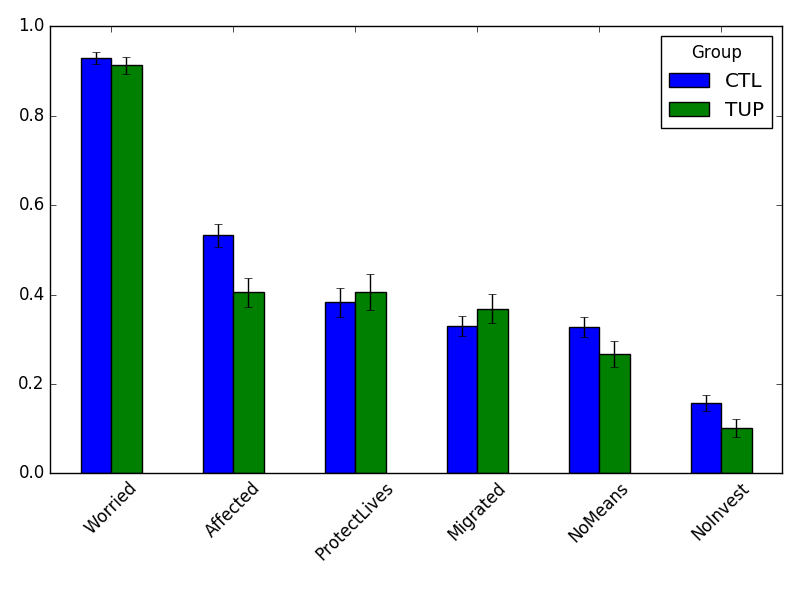
\includegraphics[width=.9\linewidth]{../figures/conflict_exposure.png}
\caption{\label{fig:conflict_exposure}\% of Sample reporting exposure to conflict by group.}
\end{figure} 

\begin{longtable}{lrrrrrrr}
\caption{\label{tab:Income}Average treatment effects by group-year on the probability of having been affected in a significant way by the outbreak of violence in late 2013}
\\
\hline
 & Affected & Migrated & NoInvest & NoMeans & ProtectLives & Worried\\
\hline
\endhead
\hline\multicolumn{7}{r}{Continued on next page} \\
\endfoot
\endlastfoot
CTL mean & \$ 0.53$^{\textbf{*}}$\$ & \$ 0.33$^{\textbf{*}}$\$ & \$ 0.16$^{\textbf{*}}$\$ & \$ 0.33$^{\textbf{*}}$\$ & \$ 0.38$^{\textbf{*}}$\$ & \$ 0.93$^{\textbf{*}}$\$\\
 & $( 0.03)$ & $( 0.02)$ & $( 0.02)$ & $( 0.02)$ & $( 0.03)$ & $( 0.01)$\\
TUP & $-0.13^{***}$ & \$ 0.04\$ & $-0.06^{**}$ & $-0.06$ & \$ 0.02\$ & $-0.02$\\
 & $( 0.04)$ & $( 0.04)$ & $( 0.03)$ & $( 0.04)$ & $( 0.05)$ & $( 0.02)$\\
\hline
F-stat & \$ 9.20\$ & \$ 0.96\$ & \$ 3.95\$ & \$ 2.55\$ & \$ 0.19\$ & \$ 0.49\$\\
N & $601.00$ & $655.00$ & $655.00$ & $655.00$ & $585.00$ & $603.00$\\
\hline
\end{longtable}

\newpage
\section{Concluding Remarks}
\label{sec-4}

BRAC's South Sudan pilot of the TUP program represents the only such test of the
ultra-poor graduation framework conducted in an area of significant political and
economic instability. It also represents among the only direct comparisons of this
model to a similarly expensive unconditional cash transfer, arguably its most
sensible benchmark for success. As such, it provides suggestive evidence as to the
best way of transfering wealth in order to help poor and vulnerable households.

Cash transfers appear to increase consumption and possibly shift investment from
agriculture to non-farm activities, without a related increase in wealth or income.
Conversely, the TUP program increased wealth and directly shifted work from
agriculture to livestock, with increased consumption in the short run. We also find
that having received asset transfers dampened the negative investment effects
following the outbreak of violence. \footnote{Whether a cash transfer would have had a
similar mitigating effect is hard to say.} We tentatively conclude that targeted
asset transfers can play a constructive role in helping poor, self-employed
households when they face economic uncertainty. And while cash increases household
consumption, the goal of improving income or wealth is aided by the additional
services that the ultra-poor graduation framework offer.
% Emacs 24.5.1 (Org mode 8.2.10)
\end{document}
